\documentclass[sans serif,9pt,xcolor=dvipsnames]{beamer}%tipo de documento

\usetheme{Copenhagen}% tema a utilizar
%\useoutertheme{infolines}
%\usecolortheme[RGB={50,93,16}]{structure}
\usecolortheme[RGB={123,16,64}]{structure}
\useinnertheme{rectangles}
%79 168 51
\setbeamercovered{transparent}
%para el difumidado de las transparencias
\beamertemplateshadingbackground{gray!20}{purple!20}
% papaquetes personales
\usepackage[spanish]{babel}%paquete de idioma
%la utilizacion de la instruccion anterior puede llevar a que existan errores en los demás paquetes para ello:
\renewcommand{\contentsname}{Contenido}
\renewcommand{\partname}{Parte}
\renewcommand{\appendixname}{Apéndice}
\renewcommand{\figurename}{Figura}
\renewcommand{\tablename}{Tabla}
\renewcommand{\abstractname}{Resumen}

\usepackage[utf8]{inputenc}% utf8 permite la utilizacion de tildes y Ñ directamente del teclado si la distribucion es utf8. Pero si se tiene otra distribucion, el argumento será latin1
\usepackage{geometry} % para margenes
\usepackage{graphicx} % para colocacion de figuras
\usepackage{color}% para colorear el texto
\usepackage{hyperref}%para hacer referencias a las direcciones de paginas en internet
\usepackage{url}% para escribir una URL
\usepackage{ragged2e}

\begin{document}
\title[\LaTeX]{\textbf{\Huge Programación Literaria Investigación Reproducible y Software Libre}}  
\author[Ing. Milton Labanda, Mg.]{Ing. Milton Labanda, Mg.}
\institute[UIDE Informática]{Carrera de Ingeniería Informática y Multimedia\\ Universidad Internacional del Ecuador}

\setbeamerfont{title}{shape=\itshape,family=\rmfamily}%cambiar tipo de letra
%\setbeamercolor{title}{fg=blue!80!black,bg=green!20!white}%comabiar color de letra y color de cuadro

%marco para el pie en el titulo
\begin{frame}
%
\includegraphics[height=0.2\textheight]{imagenes/escudoUNL.png} 
%\hfill 
\includegraphics[height=0.2\textheight]{imagenes/logoSIS.png}
\hfill {Reunión Nacional de Ramas IEEE RNR2015}
\titlepage
\begin{center}
%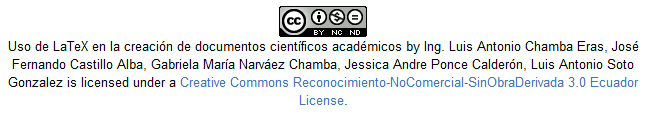
\includegraphics[height=0.2\textheight]{imagenes/licencia.PNG} 
\end{center}

\end{frame}

%marco para el contenido
\AtBeginSection [<+-| alert@+>]{
\begin{frame}{Outline} %<beamer>
\frametitle {Contenido}
\tableofcontents [currentsection]
\end{frame}}

%\logo{
\includegraphics[[width=0.7\paperwidth, height=0.7\paperheight]{imagenes/cis} }
%\setbeamertemplate{background canvas} {
\includegraphics[width=\paperwidth,height=\paperheight]{imagenes/cis}}



\section{Programación Literaria}
\subsection{Historia}
\begin{frame}
\frametitle{Historia}
\begin{block}{Como empieza todo?}
\begin{columns}
\column{.1\textwidth} \hspace{0.7cm}
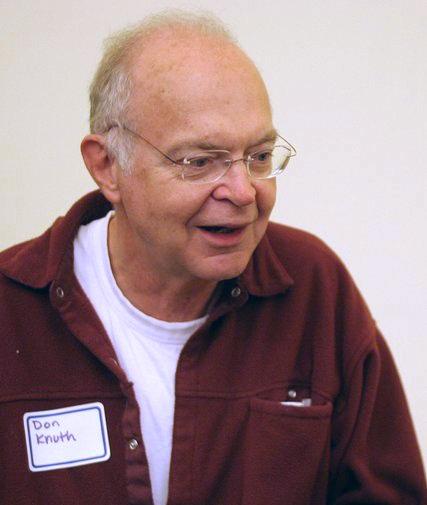
\includegraphics[width=1.8cm]{imagenes/donald.jpg}
\column{.8\textwidth}
\justifying
"I believe that the time is ripe for significantly better documentation of programs, and that we can best achieve this by considering programs to be works of literature. Hence, my title: "Literate Programming" \textbf{\textit{Donald Knuth}}
\end{columns}
\end{block}

\begin{block}{El objetivo}
\begin{columns}
\column{.1\textwidth} \hspace{0.7cm}
%\includegraphics[height=1.5cm]{imagenes/images.png} 
\column{.8\textwidth}
\justifying
Computer programs should be written in a combination of the programming language (the usual source code) and the natural language, which explains the logic of the program. \textbf{\textit{Donald Knuth}}
\end{columns}
\end{block}

\end{frame}

\begin{frame}
\frametitle{Historia}
\begin{block}{Enfoque}
\begin{columns}
\column{.1\textwidth} \hspace{0.7cm}
% % %
\includegraphics[width=1.8cm]{imagenes/latex.png} 
\column{.8\textwidth}
\justifying
El enfoque de la programación Literaria es contrario al de la programación tradicional: En vez de escribir código que contiene documentación el programador literario escribe documentación que contiene código.
\end{columns}
\end{block}
\end{frame}

\subsection{?`Qué es  \LaTeX ?}
\begin{frame}
  \frametitle{?`Qué es  \LaTeX ?}
\begin{itemize}
\justifying
\item LaTeX es un sistema de preparación de documentos de alta calidad especialmente diseñado para la producción de documentos científicos y técnicos, aunque puede utilizarse para casi para cualquier tipo de publicación. Está disponible para casi todas las plataformas existentes, y sus archivos se pueden intercambiar con facilidad entre ellas. 
\bigskip
\item La combinación de alta calidad de los resultados, gratuidad, disponibilidad y compatibilidad ha contribuido a su amplia difusión,  especialmente entre la comunidad científica convirtiéndose en estándar para la elaboración, comunicación y publicación de documentos científicos.
\end{itemize}
\end{frame}

\subsection{?`Por qué utilizar \LaTeX ?}
\begin{frame}
  \frametitle{?`Por qué utilizar \LaTeX ?}
\begin{itemize}
\justifying
\item \LaTeX  distribuye  el texto de manera adecuada, dando al conjunto una apariencia elegante similar a la de un libro.\pause
\item Los procesadores de texto no trabajan muy bien con fórmulas, en cambio LATEX hace este proceso a la perfección.\pause
\item \LaTeX es una potente herramienta para la escritura de documentos  complejos como libros o artículos científicos.\pause
\item El diseño lógico con que trabaja \LaTeX, permite una composición detallada  del documento
\end{itemize}
\end{frame}

\section{Distribuciones}
\begin{frame}
\frametitle {Distribuciones \TeX}
\justifying
Una distribución integra todo lo necesario para que funcione  \TeX y \LaTeX sobre un sistema operativo. Contiene el núcleo principal del programa, paquetes y extensiones adicionales.

\begin{block}{Linux}
\begin{itemize}
\justifying
\item \textbf{Distribución:} \textcolor{brown}{\textbf{TeXLive}} version actual 2011\\
\item Proporciona un sistema integral de TeX con los binarios para la mayoría de las variantes de Unix, como GNU / Linux, y también de Windows. 
Incluye los programas relacionados con \TeX, paquetes macro, y las fuentes que son software libre, incluyendo soporte para varios idiomas\\
\item \textbf{Enlace de Descarga:}\\
Manualmente\hfill \textcolor{blue}{\url{http://www.tug.org/texlive/}}\\
Internet\hfill sudo apt-get install texlive-full \\
\hfill sudo apt-get install texlive
\end{itemize}
\end{block}
\end{frame}


\begin{frame}
\frametitle{Distribuciones \TeX }

\begin{block}{Windows}
\begin{itemize}
\justifying
\item \textbf{Distribución: } \textcolor{brown}{\textbf{MikTeX}} version actual 2.9
\item Actualización automática, MikTeX descarga nuevas versiones de componentes y paquetes instalados previamente. Su código es abierto.
Posee convertidores para generar archivos PostScript (.ps), .pdf, .html,etc.
\item \textbf{Enlace de Descarga: }\textcolor{blue}{\url{http://www.miktex.org/2.9/setup}}
\end{itemize}
\end{block}
\end{frame}

\begin{frame}
\frametitle{Distribuciones \TeX }
\justifying
\begin{block}{Mac OS}
\begin{itemize}
\item \textbf{Distribución: } \textcolor{brown}{\textbf{ MacTeX}} version actual 2011
\item Es una redistribución de TeXLive que está dedicado exclusivamente para utilidades Mac. MacTeX es empaquetado y distribuido por el grupo de trabajo MacTeX TeXnical.
\item \textbf{Enlace de Descarga: }\textcolor{blue}{\url{ http://www.tug.org/mactex/2011/ }}
\end{itemize}
\end{block}
\end{frame}

\section{Editores \LaTeX}
\begin{frame}
\frametitle {Editores \LaTeX}
\justifying


\begin{block}{TeXMaker}
\begin{columns}
\column{.1\textwidth} \hspace{0.7cm}

\includegraphics[width=1.8cm]{imagenes/texmaker.png} 
\column{.8\textwidth}
\begin{itemize}
\justifying
\item Versión 3.3.3  abril 2012
\item Editor gratuito y multiplataforma. Liberado bajo la licencia GPL
\item Integración de las herramientas necesarias para desarrollar documentos con LaTeX, en una sola aplicación. 
\item Incluye soporte Unicode, revisión ortográfica, plegado de código y un visor de pdf y modo de visualización continua.
\item \textbf{Enlace de Descarga:}\textcolor{blue}{\url{http://www.xm1math.net/texmaker/}}
\end{itemize}
\end{columns}
\end{block}
\justifying
\textbf{Opciones:} Kile(Linux),WinShell(windows),Smultron,Scribo,TeXworks, Fraise,Latexian.
\end{frame}


\begin{frame}
\frametitle {Editores \LaTeX \hspace{0.1cm}  con Interfaz Gráfica}
\begin{block}{LyX}
\begin{columns}
\column{.1\textwidth} \hspace{0.7cm}

\includegraphics[width=1.8cm]{imagenes/lyx.PNG} 
\column{.8\textwidth}
\begin{itemize}
\justifying
\item Version 2.0.3  marzo del 2012
\item Principal característica es la interfaz gráfica.
\item Enfoque basado en la estructura del documento y no simplemente en su aspecto.
\item Tiene un editor de ecuaciones totalmente integrado para la creación de contenido matemático
\item LyX se publica bajo una licencia Free Software / Open Source, funciona en Linux/Unix, Windows y Mac OS X, y está disponible en varios idiomas.
\item \textbf{Enlace de Descarga:}\textcolor{blue}{\url{http://www.lyx.org/WebEs.Download}}
\end{itemize}
\end{columns}
\end{block}

\end{frame}

\section{\LaTeX en la web}
\begin{frame}
\frametitle {\LaTeX \hspace{0.1cm}  en la web}
\begin{block}{ScripTeX}
%\begin{columns}
%\column{.1\textwidth} \hspace{0.6cm}
\hfill 
\includegraphics[width=1.4cm]{imagenes/scribtex.jpg} 
%\column{.8\textwidth}
\begin{itemize}
\justifying
\item Funcionalidades: almacenar en nuestra cuenta los documentos creados de forma permanente o compartirlos con otros usuarios para trabajar en equipo.
\item Compatible con dispositivos móviles como el iPhone y iPad
\item Opción de trabajo en línea ideal cuando el software habitual falla
\item \textbf{Enlace}\textcolor{blue}{\url{https://www.scribtex.com/}}
\end{itemize}
%\end{columns}
\end{block}
\end{frame}

\begin{frame}
\frametitle {\LaTeX \hspace{0.2cm} en la web}

\begin{block}{Editor Online de Ecuaciones \LaTeX}
\justifying
Este programa permite practicar lo básico del código LaTeX, muestra en tiempo real el aspecto gráfico que tomarán las expresiones algebraicas
Editor de ecuaciones que genera ecuaciones gráficas (gif, png, swf, pdf, emf).\\
\textbf{Enlace: }\textcolor{blue}{\url{http://rinconmatematico.com/latexrender/}}
\end{block}

\end{frame}

\section{Plug-in para tablas desde Calc}
\begin{frame}
\frametitle {Plug-in para tablas desde Calc}
\justifying
LaTeX puede reutilizar los datos existentes en tablas creadas con las hojas de cálculo de OpenOffice, mediante la macro \textcolor{brown}{\textbf{ Calc2latex}}\\

\textbf{Enlace de Descarga: }\textcolor{blue}{\url{http://calc2latex.sourceforge.net/}}
\end{frame}

\section{Creación de Documentos en \LaTeX}
\begin{frame}
\frametitle {Creación de Documentos en \LaTeX}
\begin{center}
\begin{columns}
\column{.2\textwidth} \hspace{1 cm}

\textbf{Tipos de Documentos:}
\begin{enumerate}
\item beamer
\item articulo
\item report
\item letter
\item book
\end{enumerate}
\column{.8\textwidth}
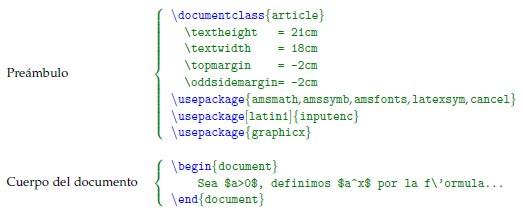
\includegraphics[height=4cm]{imagenes/estDoc.PNG}  
\end{columns}
\end{center}

\end{frame}

\begin{frame}
\frametitle {Creación de Documentos en \LaTeX : Plantillas}
\begin{enumerate}
\item Artículos Científicos
\item Presentaciones
\item Póster
\item Libros
\item Proyectos de Fin de Carrera 
\item Memorias Técnicas
\item Tesis Doctoral
\end{enumerate}
\end{frame}

\section{\LaTeX  en dispositivos portables}
\subsection{VerbTeX LaTex Editor}
\begin{frame}
\frametitle{\LaTeX desde dispositivos móviles}
\begin{block}{VerbTeX LaTex Editor}
\justifying
Es un editor gratuito \LaTeX de colaboración para su dispositivo Android. Te permite crear y gestionar proyectos de \LaTeX directamente en su dispositivo Android y generar un archivo PDF utilizando el servicio de \LaTeX disponible en \textcolor{blue}{\url{http://www.verbosus.com}}  
\end{block}
\begin{center}
\begin{columns}
\column{.2\textwidth} \hspace{0.7cm}

\includegraphics[width=2.5 cm]{imagenes/verbtex.jpg} 
\column{.10\textwidth}
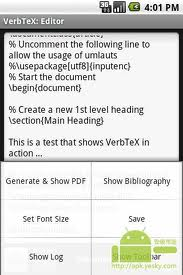
\includegraphics[width=2.5 cm]{imagenes/movilVerbtex.jpg} 
\end{columns}
\end{center}




\end{frame}

\begin{frame}
\frametitle{\LaTeX desde dispositivos móviles}


\begin{block}{ VerbTeX LaTeX Editor: Enlaces de Descarga}
\begin{itemize}
\justifying
\item \textit{Desde el ordenador:}  \textcolor{blue}{\url{http://www.verbosus.com/VerbTeX_v2.1.9.apk}}
\item \textit{Desde el Movil:} 
\begin{itemize}
\justifying
\item Versión Gratuita:\textcolor{brown}{\textbf{VerbTeX LaTeX Editor}}\hfill \textcolor{blue}{\url{Link https://play.google.com/store/apps/details?id=verbosus.verbtex&feature=search_result }}
\item Versión de Pago:\textcolor{brown}{\textbf{VerbTeX Pro LaTeX (Encryption) 1.49 euro }}  \hfill \textcolor{blue}{\url{https://play.google.com/store/apps/details?id=verbosus.verbtexpro&feature=search_result }}
\end{itemize}
\end{itemize}
\end{block}

\end{frame}

\begin{frame}
\frametitle {Versiones de VerbTeX LaTex Editor}
\begin{center}
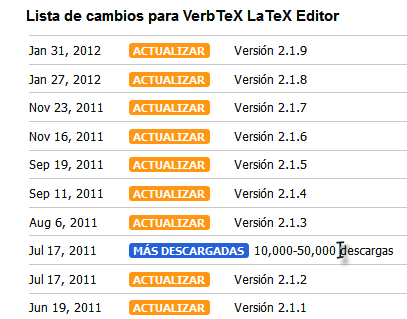
\includegraphics[height=4cm]{imagenes/vMobil.png} 
\end{center}
\justifying
\textbf{Detexify Latex Recognizer}\\
\textit{Enlace al Google Play:}\textcolor{blue}{\url{https://play.google.com/store/apps/details?id=coolcherrytrees.software.detexify&feature=search_result }}
\end{frame}

\subsection{Utilización de USBTeX}
\begin{frame}
\frametitle {Utilización de USBTeX}
\begin{center}

\includegraphics[height=1.5 cm]{imagenes/usbtex.png} 
\end{center}
\begin{block}{Ventajas de USBTEX}
\begin{itemize}
\justifying
\item Es portable(ejecutable en cualquier ordenador Windows)
\item Útil para personas que viajan constantemente
\item Viene empaquetado todas las aplicaciones(Gostscript, Ghostview, un editor y su configuración) necesarios para ejecutar 
\end{itemize}
\end{block}

\begin{block}{Inconvenientes de USBTEX}
\begin{itemize}
\justifying
\item No compila archivos Beamers
\item Solo acepta (*.eps) para imágenes y figuras
\end{itemize}
\end{block}
\end{frame}

\section{Enlaces de Ayuda}
\begin{frame}
\frametitle {Enlaces de Ayuda}
\begin{thebibliography}{10}
\bibitem{  } Alex Borbón A., Walter Mora F.
\newblock{ \LaTeX Composición, Diseño Editorial, Gráficos,
Inkscape, Tikz y Presentaciones Beame} 2012
\newblock 
\url{http://www.tec-digital.itcr.ac.cr/revistamatematica/Libros/LATEX/LaTeX_2011.pdf}

\end{thebibliography}
\end{frame}

\begin{frame}
\frametitle {Créditos}
	\begin{center}
		\textbf{\textit{Expositores}}\\
			Ing. Luis Antonio Chamba Eras\\
			José Fernando Castillo Alba\\
			Gabriela María Narváez Chamba\\
			Jessica Andrea Ponce Calderón\\
			Luis Antonio Soto  Gonzalez\\
\vspace{0.5 cm}
\textbf{\textit{Escritura Científica en \LaTeX }}\\
Grupo de Apoyo para la Escritura Científica\\
  Décimo Módulo\\
  \vspace{0.3 cm}

\includegraphics[height=0.5 cm]{imagenes/escudoUNL.png} \\
\textbf{Universidad Nacional de Loja\\
Carrera de Ingeniería en Sistemas\\
2012
}
	\end{center}
\end{frame}

\end{document}
